\documentclass[14pt]{extbook}
\usepackage{multicol, enumerate, enumitem, hyperref, color, soul, setspace, parskip, fancyhdr} %General Packages
\usepackage{amssymb, amsthm, amsmath, bbm, latexsym, units, mathtools} %Math Packages
\everymath{\displaystyle} %All math in Display Style
% Packages with additional options
\usepackage[headsep=0.5cm,headheight=12pt, left=1 in,right= 1 in,top= 1 in,bottom= 1 in]{geometry}
\usepackage[usenames,dvipsnames]{xcolor}
\usepackage{dashrule}  % Package to use the command below to create lines between items
\newcommand{\litem}[1]{\item#1\hspace*{-1cm}\rule{\textwidth}{0.4pt}}
\pagestyle{fancy}
\lhead{Progress Quiz 10}
\chead{}
\rhead{Version B}
\lfoot{}
\cfoot{}
\rfoot{Fall 2020}
\begin{document}

\begin{enumerate}
\litem{
\begin{enumerate}[label=\Alph*.]

\end{enumerate} }
\litem{
Simplify the expression below into the form $a+bi$. Then, choose the intervals that $a$ and $b$ belong to.\[ \frac{45 - 77 i}{8 - i} \]\begin{enumerate}[label=\Alph*.]
\item \( a \in [3, 4.5] \text{ and } b \in [-11, -9] \)
\item \( a \in [6, 7.5] \text{ and } b \in [-9.5, -8] \)
\item \( a \in [5, 6.5] \text{ and } b \in [76.5, 78] \)
\item \( a \in [6, 7.5] \text{ and } b \in [-572, -570] \)
\item \( a \in [435.5, 437.5] \text{ and } b \in [-9.5, -8] \)

\end{enumerate} }
\litem{
Simplify the expression below into the form $a+bi$. Then, choose the intervals that $a$ and $b$ belong to.\[ (-3 - 10 i)(8 - 2 i) \]\begin{enumerate}[label=\Alph*.]
\item \( a \in [-26, -20] \text{ and } b \in [17, 25] \)
\item \( a \in [-49, -39] \text{ and } b \in [-74, -70] \)
\item \( a \in [-4, -2] \text{ and } b \in [-86, -82] \)
\item \( a \in [-49, -39] \text{ and } b \in [66, 76] \)
\item \( a \in [-4, -2] \text{ and } b \in [83, 87] \)

\end{enumerate} }
\litem{
Simplify the expression below and choose the interval the simplification is contained within.\[ 7 - 15 \div 9 * 13 - (17 * 4) \]\begin{enumerate}[label=\Alph*.]
\item \( [-65.13, -58.13] \)
\item \( [74.87, 76.87] \)
\item \( [-91.67, -77.67] \)
\item \( [-130.67, -120.67] \)
\item \( \text{None of the above} \)

\end{enumerate} }
\litem{
Choose the \textbf{smallest} set of Complex numbers that the number below belongs to.\[ \frac{12}{8}+81i^2 \]\begin{enumerate}[label=\Alph*.]
\item \( \text{Pure Imaginary} \)
\item \( \text{Nonreal Complex} \)
\item \( \text{Not a Complex Number} \)
\item \( \text{Irrational} \)
\item \( \text{Rational} \)

\end{enumerate} }
\litem{
Choose the \textbf{smallest} set of Real numbers that the number below belongs to.\[ -\sqrt{\frac{44100}{225}} \]\begin{enumerate}[label=\Alph*.]
\item \( \text{Integer} \)
\item \( \text{Rational} \)
\item \( \text{Whole} \)
\item \( \text{Not a Real number} \)
\item \( \text{Irrational} \)

\end{enumerate} }
\end{enumerate}

\end{document}\documentclass[14pt]{extbook}
\usepackage{multicol, enumerate, enumitem, hyperref, color, soul, setspace, parskip, fancyhdr} %General Packages
\usepackage{amssymb, amsthm, amsmath, bbm, latexsym, units, mathtools} %Math Packages
\everymath{\displaystyle} %All math in Display Style
% Packages with additional options
\usepackage[headsep=0.5cm,headheight=12pt, left=1 in,right= 1 in,top= 1 in,bottom= 1 in]{geometry}
\usepackage[usenames,dvipsnames]{xcolor}
\usepackage{dashrule}  % Package to use the command below to create lines between items
\newcommand{\litem}[1]{\item#1\hspace*{-1cm}\rule{\textwidth}{0.4pt}}
\pagestyle{fancy}
\lhead{Progress Quiz 10}
\chead{}
\rhead{Version B}
\lfoot{}
\cfoot{}
\rfoot{Fall 2020}
\begin{document}

\begin{enumerate}
\litem{
Write the equation of the line in the graph below in Standard form $Ax+By=C$. Then, choose the intervals that contain $A, B, \text{ and } C$.
\begin{center}
    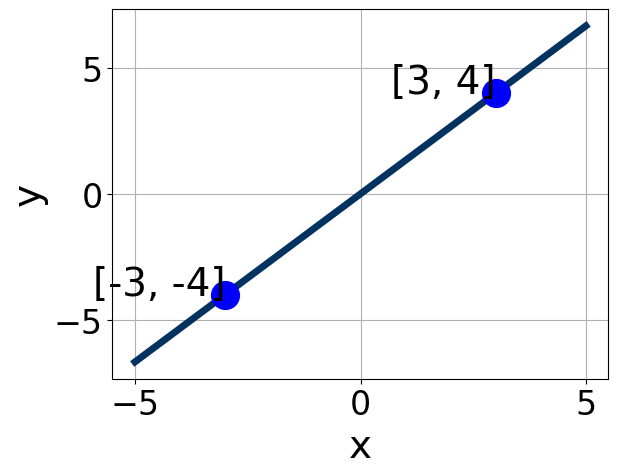
\includegraphics[width=0.5\textwidth]{../Figures/linearGraphToStandardB.png}
\end{center}
\begin{enumerate}[label=\Alph*.]
\item \( A \in [-2.8, 2.4], \hspace{3mm} B \in [-0.3, 3.7], \text{ and } \hspace{3mm} C \in [-1, 2] \)
\item \( A \in [1.8, 6.2], \hspace{3mm} B \in [-6.1, -3], \text{ and } \hspace{3mm} C \in [-1, 2] \)
\item \( A \in [-3.1, -1.9], \hspace{3mm} B \in [-6.1, -3], \text{ and } \hspace{3mm} C \in [-1, 2] \)
\item \( A \in [-2.8, 2.4], \hspace{3mm} B \in [-2.2, -0.7], \text{ and } \hspace{3mm} C \in [-1, 2] \)
\item \( A \in [1.8, 6.2], \hspace{3mm} B \in [3.5, 5.9], \text{ and } \hspace{3mm} C \in [-1, 2] \)

\end{enumerate} }
\litem{
Find the equation of the line described below. Write the linear equation as $ y=mx+b $ and choose the intervals that contain $m$ and $b$.\[ \text{Parallel to } 9 x - 5 y = 11 \text{ and passing through the point } (-10, 3). \]\begin{enumerate}[label=\Alph*.]
\item \( m \in [1.8, 4.8] \hspace*{3mm} b \in [9, 17] \)
\item \( m \in [1.8, 4.8] \hspace*{3mm} b \in [-21, -20] \)
\item \( m \in [-0.44, 1.56] \hspace*{3mm} b \in [18, 24] \)
\item \( m \in [1.8, 4.8] \hspace*{3mm} b \in [18, 24] \)
\item \( m \in [-1.8, 0.2] \hspace*{3mm} b \in [-16, -14] \)

\end{enumerate} }
\litem{
First, find the equation of the line containing the two points below. Then, write the equation as $ y=mx+b $ and choose the intervals that contain $m$ and $b$.\[ (-5, 10) \text{ and } (-11, 7) \]\begin{enumerate}[label=\Alph*.]
\item \( m \in [0.1, 1.5] \hspace*{3mm} b \in [-13.53, -11.48] \)
\item \( m \in [0.1, 1.5] \hspace*{3mm} b \in [13.6, 15.03] \)
\item \( m \in [0.1, 1.5] \hspace*{3mm} b \in [16.89, 18.44] \)
\item \( m \in [-1.7, 0.4] \hspace*{3mm} b \in [1.08, 1.63] \)
\item \( m \in [0.1, 1.5] \hspace*{3mm} b \in [12.18, 12.84] \)

\end{enumerate} }
\litem{
\begin{enumerate}[label=\Alph*.]

\end{enumerate} }
\litem{
Solve the equation below. Then, choose the interval that contains the solution.\[ -9(5x -17) = -15(-13x -8) \]\begin{enumerate}[label=\Alph*.]
\item \( x \in [-0.34, 0.35] \)
\item \( x \in [1.77, 2.37] \)
\item \( x \in [0.23, 0.77] \)
\item \( x \in [-4.28, -3.46] \)
\item \( \text{There are no real solutions.} \)

\end{enumerate} }
\litem{
Solve the linear equation below. Then, choose the interval that contains the solution.\[ \frac{-7x + 8}{3} - \frac{5x -7}{7} = \frac{-3x -6}{2} \]\begin{enumerate}[label=\Alph*.]
\item \( x \in [12.85, 13.83] \)
\item \( x \in [4.08, 4.44] \)
\item \( x \in [2.27, 3.62] \)
\item \( x \in [0.1, 0.97] \)
\item \( \text{There are no real solutions.} \)

\end{enumerate} }
\end{enumerate}

\end{document}